To introduce the \textbf{Fisher Information} (FI), we will start off with how it is defined and used in statistics.\\
Let's look at a statistical model $f(x_i|\theta)$ that represents how a parameter $\theta$ is related to the outcomes $x_i$ of random variables $X_i$\cite{StatisticFisherInfoTutorial}. As an example of what this means, let us look at the statistical model of a Galton board. For readers who are not familiar with a what Galton boards are, there is an example photograph in \cref{fig:GaltonPicture}. 
\begin{figure}
	\centering
	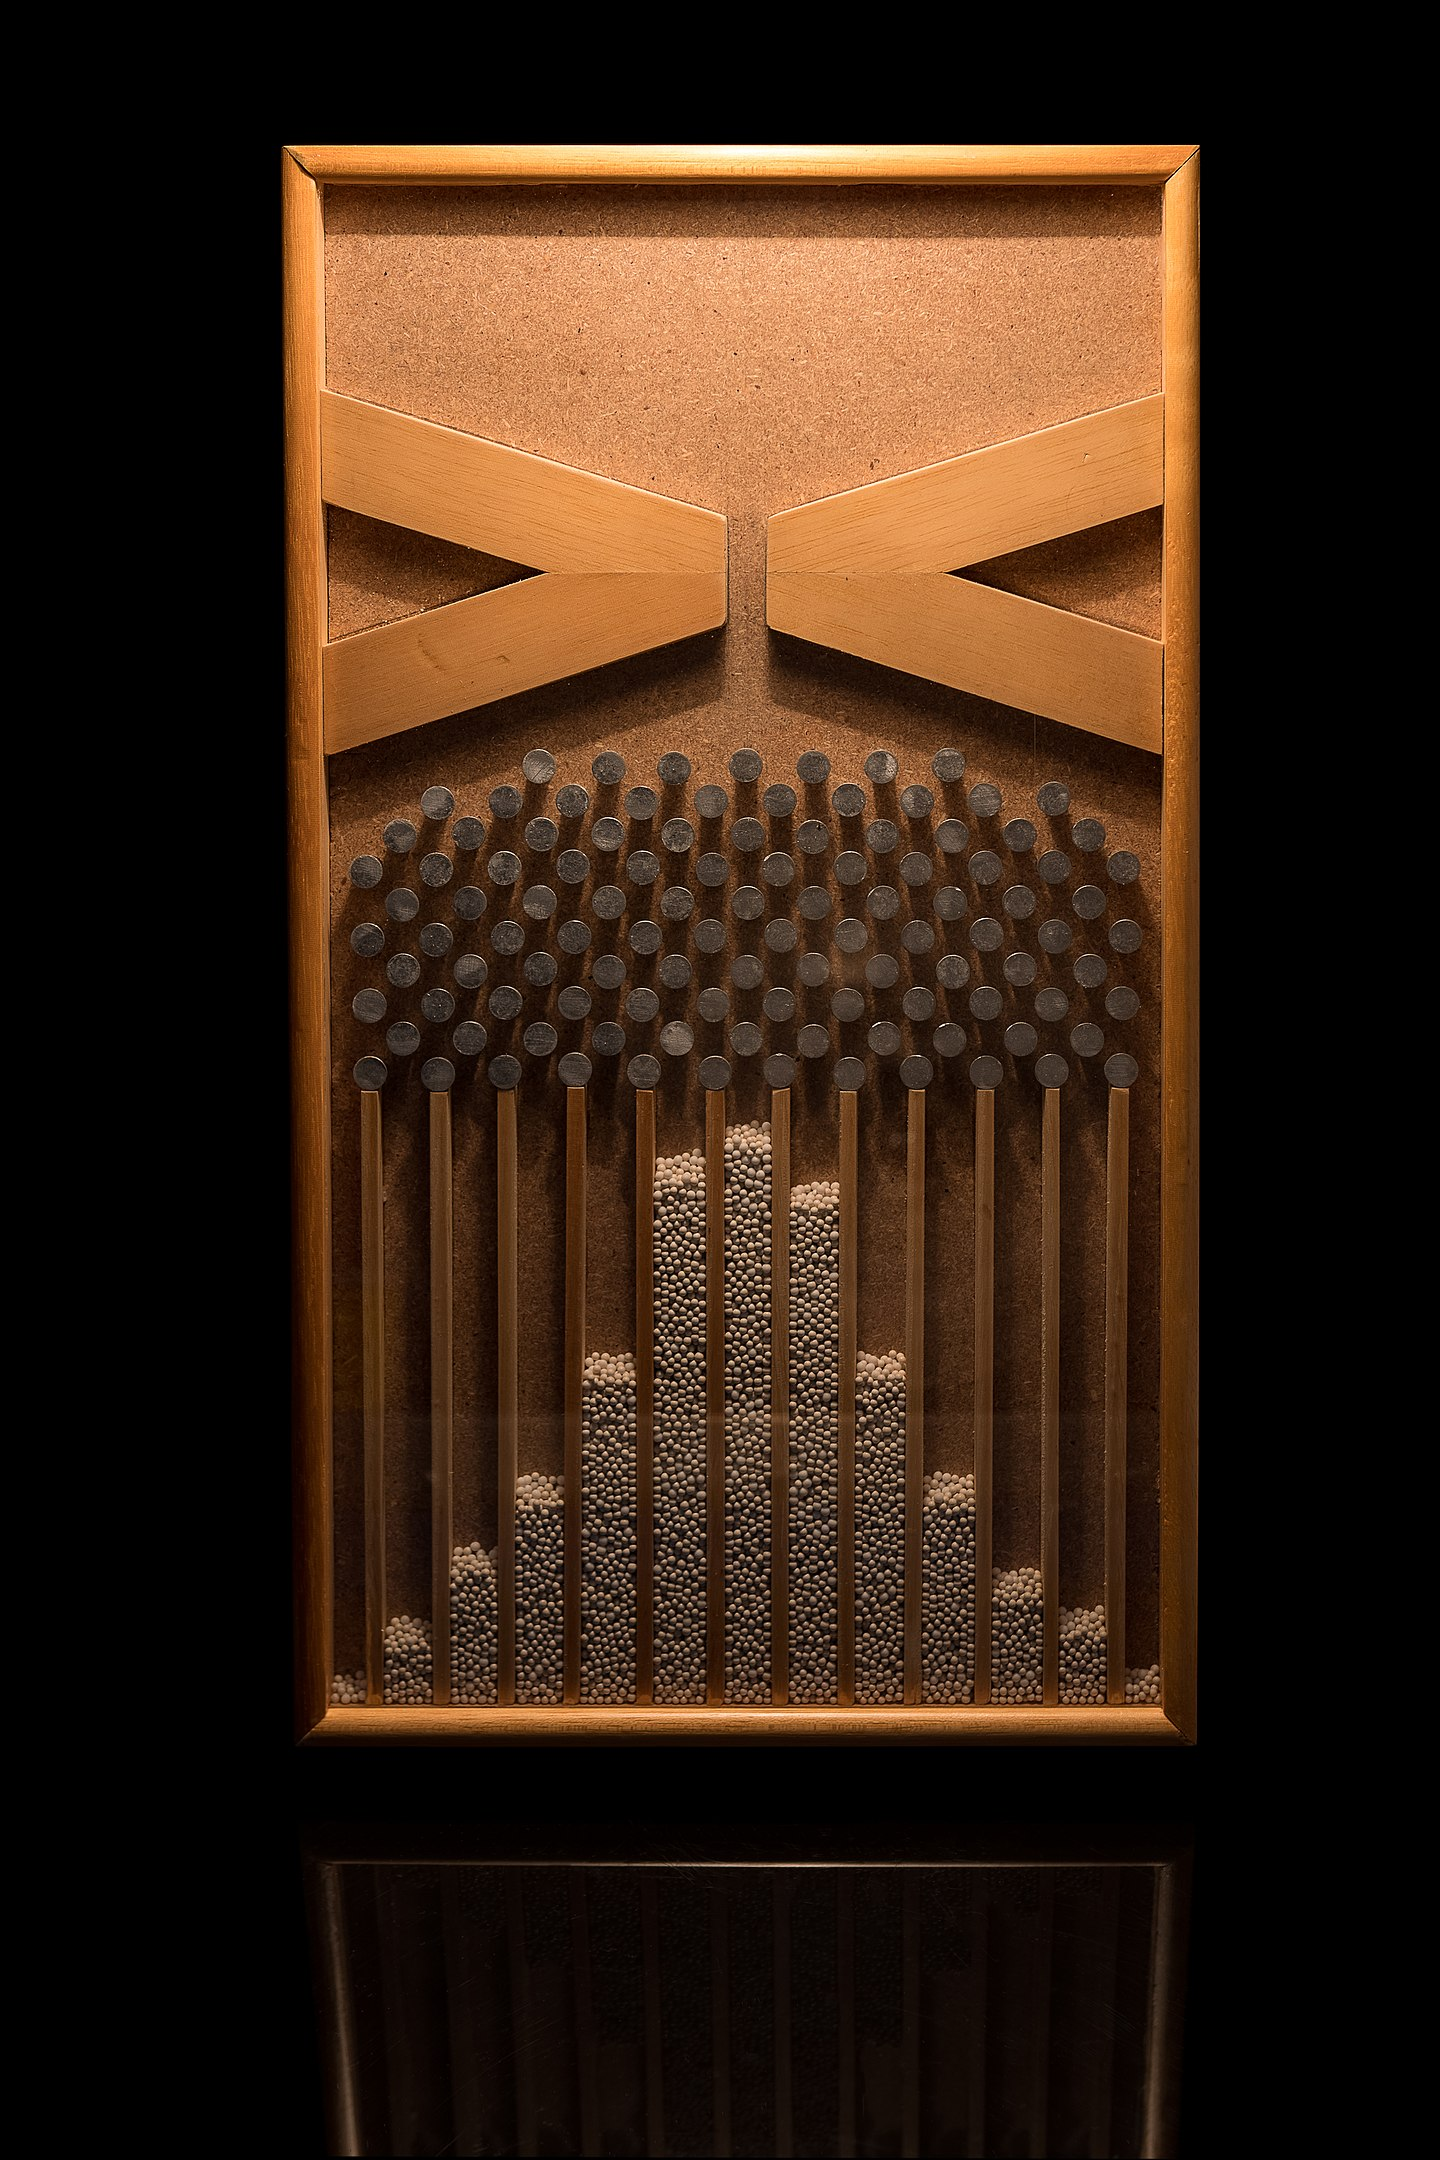
\includegraphics[width = 4cm]{text/FisherInformation/plots/GaltonBoard.jpg}
	\caption{This figure shows a picture of a Galton board. Taken from \cite{GaltonBoardPicture}.}
	\label{fig:GaltonPicture}
\end{figure}
It's a famous mechanical model that visualizes binomial distributions, which are approximations of the normal distribution. If we place many balls at the top of the board and let them fall to the bottom, the amount of balls that end up in each cell are distributed according to the binomial distribution. In this case, $x_i$ could assume the slot number which a ball can fall into. The $i$ could label multiple throws into the board, but for now we'll assume that there is only one experiment $i$. To introduce a parameter that influences the distribution of balls, let's say one can throw from different spots above the Galton board which we now control with the the value of $\theta$. For a known $\theta$, the resulting value of the statistical model represents the probability distribution $f(x_i|\theta) = p_\theta(x_i)$ for the probability of the different $x_i$ outcomes. A visual representation of the probability distributions for different $\theta$ can be seen in \cref{fig:GaltonDistributions}.
\begin{figure}
	\centering
	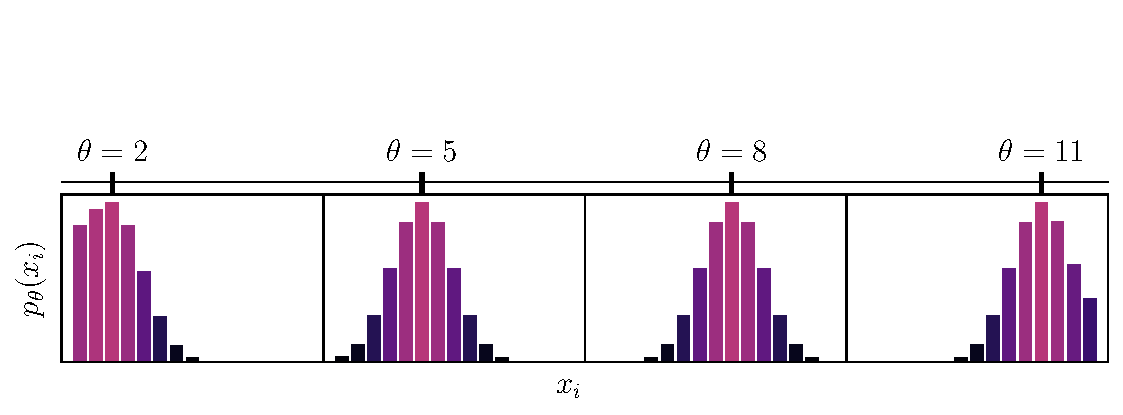
\includegraphics[width = \textwidth, clip, trim= 0cm 0cm 0cm 2.3cm]{text/FisherInformation/plots/GaltonDistributionsPlot.pdf}
	\caption{This figure shows the probability distributions for a Galton boards with different drop-in positions. The slots where the ball can end up are labeled by the value of $x_i$.}
	\label{fig:GaltonDistributions}
\end{figure}\\
In general, the statistical models might be more complex, where $\theta$ contains several parameters, $x$ being an element of a mathematical space other than $\mathbb{R}$ and the index $i$ denoting various different experiments, all depending on the same parameter, but having different possible outcomes and probability distributions.\\
What's of interest for the FI are cases where the parameters are not known before conducting the experiment, and have to be approximated by the different outcomes $x_i$.\\

Before we introduce the FI, let's look at an example from \cite{StatisticFisherInfoTutorial}. Let's consider a biased coin where we denote the probability of heads ($x_i = 1$) with $\theta$ and the probability of tails ($x_i = 0$) with $1-\theta$. We will now take a look at the outcome of $n$ tosses, represented by the variable $X^n$. For example, an observed result for $X^5$ could be $x^5 = (1,1,0,1,0)$. Let's consider another variable $Y$, whose observation is the sum of the total head throws $y = \sum x^n$. In our example case of $x^5 = (1,1,0,1,0)$, this would result in a value of $y = 3$. The probability for this variable $y$ is distributed according to the binomial distribution $f(y|\theta) = \binom{n}{y}\theta^y (1-\theta)^{n-y}$. Here the binomial coefficient $\binom{n}{y}$ represents the different combinations that result in the same value of $y$. This is needed because there are $2^n$ different possibilities for $x$, while there are only $n$ different possibilities for $y$.\\
If we now fix the outcome of $y$ and look at the conditional probability for the different $x^n$ that could have resulted in that $y$ value, we get $p(x|y,\theta) = 1/ \binom{n}{y}$. With $p(x|y,\theta)$ we denote the probability depending on $x$ for fixed $y$ and $\theta$. Although the probability of $y$ and $x$ both depend on $\theta$, the probability for $x$ when $y$ is fixed doesn't. After measuring $y$ there is no information about $\theta$ left in the measurement of $x$. This means that $y$ is fully descriptive of or "sufficient for" the parameter $\theta$. Measuring $y$ results in the same amount of information about the parameter $\theta$ as measuring the whole observation $x$. To quantify how much information a certain function of outputs $t(x)$, which is $y(x^n)$ in our example, contains about the parameters $\theta$, Fisher introduced the Fisher information.\\
The Fisher information is defined as 
\begin{equation}\label{eq:FIDefinition}
	I_{X,ij}(\theta) = \underset{x\in X}{E} \left[\tAbl{}{\theta_i}\log f(x|\theta) \cdot \tAbl{}{\theta_j}\log f(x|\theta)\right],
\end{equation}
where we used the expectation $E$
\begin{equation}
	\underset{x\in X}{E} \left[A(x)\right] = 
	\begin{cases}
		\sum_{x\in X} \left(A(x) p(x)\right) &\text{if $X$ is discrete},\\
		\int_{x\in X} A(x) p(x) \mathrm{d}x &\text{if $X$ is continuous}.
	\end{cases}
\end{equation}
Since the Fisher information is dependent of $\theta$, we can assume the value of $\theta$ to be fixed during calculation, which makes $f(x|\theta)$ equal to $p_\theta(x)$.\\ 
For $n$ independent experiments $X^n$, where $f(x^n|\theta) = \prod_{i=1}^n f(x_i|\theta)$, one can split the FI into 
\begin{equation}\label{eq:FIforIndependentExperiments}
	I_{X^n,ij}(\theta) = \prod_{i=1}^n I_{X_i,ij}(\theta).
\end{equation}
A proof of this can be found in \cref{sec:ProofFIforIndependentExperiments}.\\
For our example the FI yields $I_{X^n}(\theta) = I_{Y}(\theta) = n/(\theta(1-\theta))$\cite{StatisticFisherInfoTutorial}. This means that there is as much information about the $\theta$ contained in the measurement of $Y$ as in the measurement of $X^n$, which coincides with $Y$ being a sufficient measurement for $\theta$. \\
To conclude this chapter, the Fisher information is used in statistics to measure the amount of information one can gather about a parameter $\theta$ by measuring the outcome of a probability distribution $p_\theta(x_i)$. It is defined in equation \cref{eq:FIDefinition}.
